\section{Requirements}
\label{requirements}



In this section the requirements realised by the system are listed. The enumeration mirrors the requirement list defined in \cite{Votes14}. The identifications numbers are identical. Requirements that are not completely implemented are left out.

% TODO: remove MANDATORY... and add if realized. Maybe with short description.

\subsection{Functional Requirements}

\begin{figure}
\centering
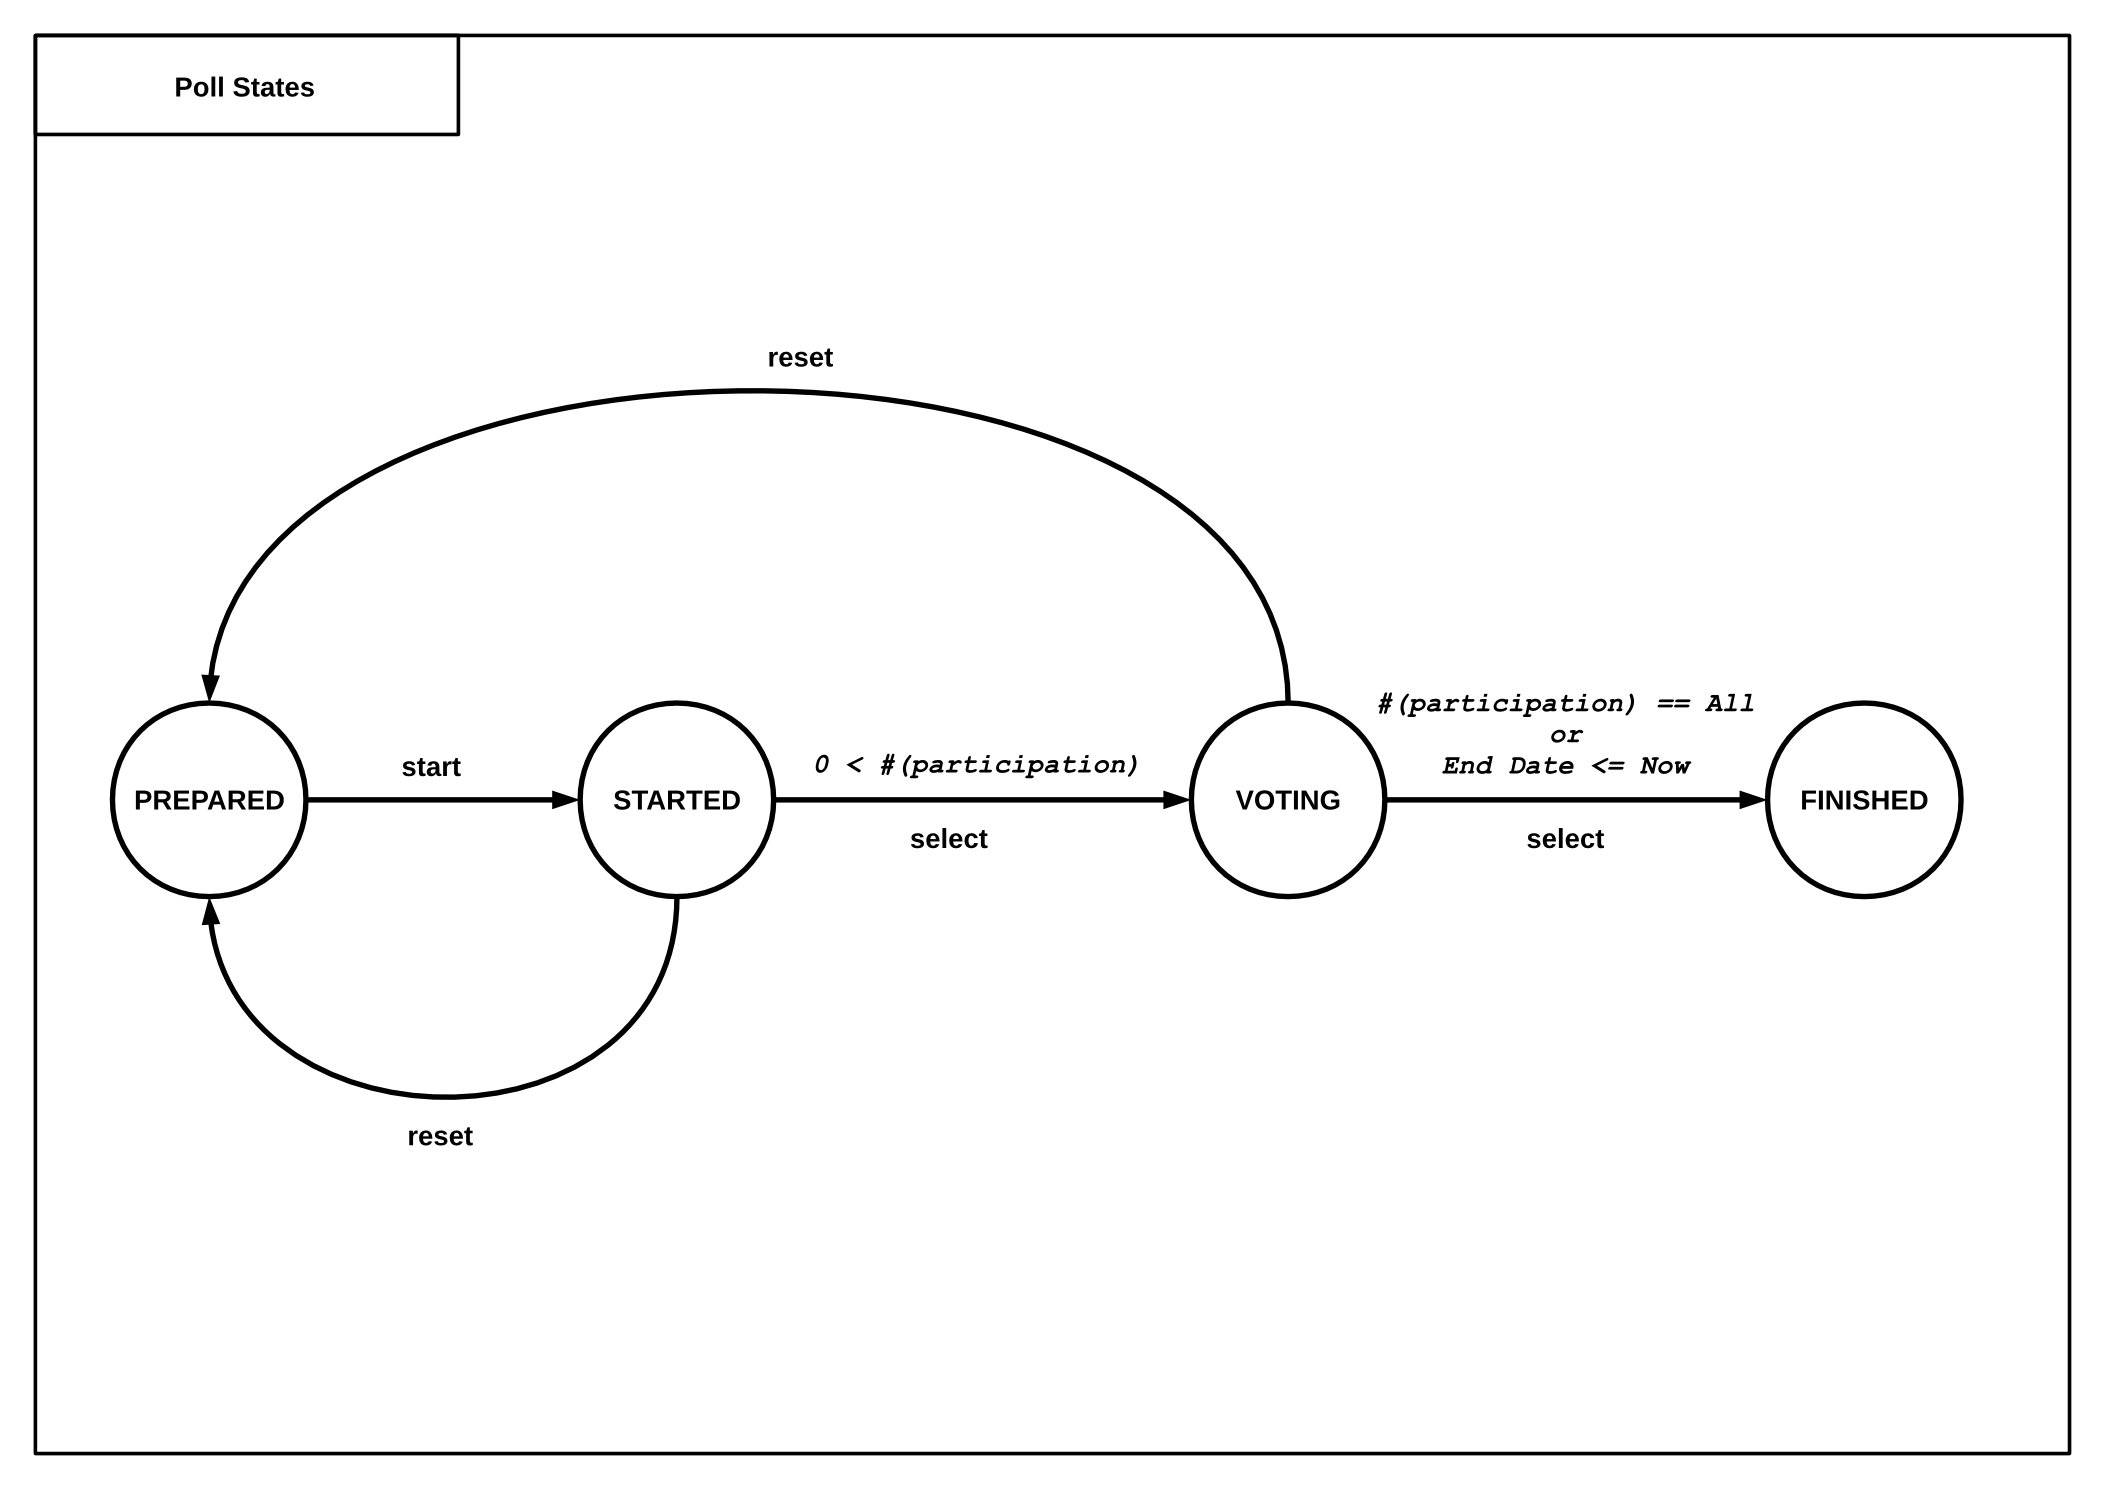
\includegraphics[width=0.9\textwidth]{png/poll-states.png}
\caption{Poll States}
\label{figure:poll-states}
\end{figure}

\begin{enumerate}

\item[1.] Polls

	\begin{enumerate}
	\item
	[1.1.] The system must support electronic polls with one or more items. MANDATORY
	
	
	\item
	[1.2.] Each poll must have a title. The title has to be unique (scope is system). MANDATORY
	
	
	\item
	[1.3.] Each poll must have a description. MANDATORY
	
	
	\item
	[1.4.] Each poll must have a voting period (start and end date with time). MANDATORY
	
	
	\item
	[1.5.] Each poll must have at least one item. MANDATORY
	
	
	\item
	[1.6.] The system must allow to group arbitrary many items into one poll. MANDATORY
	
	\end{enumerate}




\item[2.] Poll states

	\begin{enumerate}
	\item
	[2.1.] The system must implement poll states. Polls be in one of four states: PREPARED, STARTED,
	VOTING, FINISHED. State changes are specified in figure \ref{figure:poll-states}. MANDATORY
	
	
	\item
	[2.2.] When all participants submitted their votes, the system must set the poll to FINISHED.
	MANDATORY
	
	
	\item
	[2.3.] An organizer must be able to extend the voting period when a poll is in state STARTED or
	VOTING. OPTIONAL
	\end{enumerate}




\item[3.] Organizers

	\begin{enumerate}
	\item
	[3.1.] The system must allow all university members to act as organizers. MANDATORY
	
	
	\item
	[3.2.] Organizers must identify themselves with username and password. MANDATORY
	
		\begin{enumerate}
		
		
		\item
		[3.2.1.] University members can be identified by the LDAP service provided by the GHRKO
		computing center. OPTIONAL
		
		
		\item
		[3.2.2.] If LDAP is not used, an administrator must be able to create organizer accounts. OPTIONAL
	
		\end{enumerate}
	
	
	
	
	\item
	[3.3.] An organizer must be able to conduct arbitrary many polls. MANDATORY
	
	
	\item
	[3.4.] The system shall provide a preview mode that allows organizers to view how their polls look
	like when a participant fills in her choices. OPTIONAL
	
	
	\item
	[3.5.] The system can provide a possibility to add further organizers to a poll. Each organizer must
	have the same options. OPTIONAL
	
		\begin{enumerate}
			\item[3.5.1.] An organizer must be able to change the organizer list.
			
			
			\item[3.5.2.] An organizer must not be able to remove herself from the organizer list.
		
		\end{enumerate}
	
	
	\end{enumerate}




\item[4.] Administrators

	\begin{enumerate}
	\item[4.1.] The system must support an administrator role. OPTIONAL
	
	
	\item[4.2.] Administrators must have the ability to delete polls (including all votes) from the system. OPTIONAL
	
	
	\item[4.3.] Administrators must not be able to view votes nor results of polls which they didn't organize.
	OPTIONAL
	
	
	\item[4.4.] Administrators must be able to create and delete user accounts, if no LDAP authentication is
	provided (see requirement XXX). OPTIONAL
	\end{enumerate}




\item[5.] Participants

	\begin{enumerate}
	\item[5.1.] The organizer of a poll must be able to invite 3 to arbitrary many participants. In polls with
	less than 3 participants, anonymity can not be asserted. MANDATORY
	
	
	\item[5.2.] Each participant must be identified by her email address. MANDATORY
	
	
	\item[5.3.] The system shall support participants from outside the university. OPTIONAL
	
	
	\item[5.4.] After a poll is STARTED by the organizer, each participant must be informed via email about
	the poll. OPTIONAL (University mail server must not be „mis-used“, it’s sufficient to display
	the mail content on a web page)
	
	
	\item[5.5.] The information mail must include the title of the poll, the start and end dates, the number of
	participants, and a token. MANDATORY
	
	
	\item[5.6.] The information can also contain a hyperlink immediately referring to the voting page with a
	pre-filled token field. OPTIONAL
	\end{enumerate}




\item[6.] Participant lists

	\begin{enumerate}
	\item[6.1.] The organizer must be able to modify the participant list until a poll is STARTED. MANDATORY
	
	
	\item[6.2.] The system can provide a means to comfortably create participant lists, e.g. by pasting
	email addresses from other applications such as spread sheets or KLIPS. OPTIONAL
	
	
	\item[6.3.] The system shall provide a means to store participant lists for easy reuse in subsequent
	polls. OPTIONAL
	
	
	\item[6.3.1.] The stored participant lists must be private to each organizer.
	
	
	\item[6.3.2.] Each stored participant list must have a unique name (scope is per organizer).
	\end{enumerate}





\item[7.] Tokens

	\begin{enumerate}
	\item[7.1.] The token must be randomly chosen. MANDATORY
	
	
	\item[7.2.] The token must be unique (scope is system). MANDATORY
	
	
	\item[7.3.] The token must be long enough to make it very very improbable that anybody can forge a
	valid token. MANDATORY
	\end{enumerate}




\item[8.] Anonymity

	\begin{enumerate}
	\item[8.1.] The system must ensure anonymity. MANDATORY (with reasonable effort)
	
	
	\item[8.2.] At any point in time it must be impossible to identify which participant submitted which vote.
	This also must to be guaranteed for polls with participation tracking. MANDATORY
	
	
	\item[8.3.] The system must ensure that a token can not be associated with a vote. MANDATORY
	\end{enumerate}



\item[9.] Participation tracking

	\begin{enumerate}
	\item[9.1.] The system must provide an option to enable participation tracking for a poll. OPTIONAL
	
	
	\item[9.2.] The system can provide an option to configure automatic reminders via E-Mail. OPTIONAL
	\end{enumerate}




\item[10.] Submitting a vote

	\begin{enumerate}
	\item[10.1.] The system must provide a web page to submit a vote. MANDATORY
	
	
	\item[10.2.] The voting page must present an input field for a participant’s token. MANDATORY
	
	
	\item[10.3.] The token input field can be pre-filled (see requirement XX). OPTIONAL
	
	
	\item[10.4.] After the token was verified, the system must display the items. MANDATORY
	
	
	\item[10.5.] The system must present a button to submit a vote. MANDATORY
	
	
	\item[10.6.] After a vote was submitted, the token used for that vote must be invalidated (i.e. it can’t be
	re-used, participants can not change their vote after submitting). MANDATORY
	
	
	\item[10.7.] The system must allow to cancel a voting (e.g. by closing the browser, or by clicking a cancel
	button). MANDATORY
	
	
	\item[10.8.] The token used in canceled voting must be re-useable later. MANDATORY
	
	
	\item[10.9.] For a canceled voting, the system must not remember any of the choices. OPTIONAL
	
	
	\item[10.10.] The system shall ensure that subsequent participants using the same browser window
	can not restore the previous choice (e.g. by the „go back“ function or by auto fill capabilities
	of browsers). OPTIONAL
	\end{enumerate}




\item[11.] Abstain from voting

	\begin{enumerate}
	\item[11.1.] The system must provide a means to abstain from voting (Enthaltung oder ungültige
	Stimme) for each item of a poll. MANDATORY
	
	
	\item[11.2.] The system can provide a means to abstain from voting for a complete poll (this is equivalent
	to abstaining from all items). OPTIONAL
	
	\end{enumerate}



\item[12.] Types of items

	\begin{enumerate}
	\item[12.1.] The system must support different types of items. MANDATORY
	
	
	\item[12.2.] The items of a poll must have a title (titles have to be unique with scope poll). MANDATORY
	
	
	\item[12.3.] The options of an item must have a short name and a description. MANDATORY
	
	
	\item[12.4.] The system must support YES/NO items. In this case, the short names of the options are
	„yes“ and „no“. MANDATORY
	
	
	\item[12.5.] The system must support 1 OF N items. Participants can choose exactly one of zwo or
	more options. MANDATORY
	
	
	\item[12.6.] The system must support M OF N items. Participants can choose at most M of two or
	more options (M $\leq$ N). OPTIONAL
	
	
	\item[12.7.] The system can support 1 OF N items with a free text option. Participants can choose one
	of the predefined options. Alternatively, they can enter a free text to indicate their choice.
	OPTIONAL
	
	
	\item[12.8.] The system can support M OF N items with up to M free text options. Participants can
	choose at most M of the predefined options. Alternatively, they can can use less than M
	predefined options an enter the rest of their choices into free text fields. OPTIONAL
	\end{enumerate}




\item[13.] Results

	\begin{enumerate}
	\item[13.1.] An organizer must be able to view the results of a poll after the voting period is FINISHED.
	MANDATORY
	
	
	\item[13.2.] Nobody must be able to view (intermediate) results in the STARTED and VOTING states.
	MANDATORY
	\end{enumerate}



\end{enumerate}

\subsection{Non-Functional Requirements}

\begin{enumerate}

\item[14.] User interface

	\begin{enumerate}
	\item[14.1.] The system can use third-party CSS libraries (such as Twitter Bootstrap) to achieve a mod-
	ern look and feel. OPTIONAL
	\item[14.2.] The system can use advanced technologies (e.g. AJAX, JavaScript) to enhance user expe-
	rience. OPTIONAL
	\item[14.3.] The system can use third-party JSF components (e.g. myFaces, richFaces). OPTIONAL
	\item[14.4.] The system must provide a user interface suitable for desktop/laptop browsers. MANDA-
	TORY
	\item[14.5.] The user interface can support multiple devices (desktop, tablet, mobile, etc.). OPTIONAL
	\item[14.6.] The user interface must be realized with JSF. MANDATORY
	\end{enumerate}

\item[15.] Security, encrypted communication

	\begin{enumerate}
	\item[15.1.] The system must store passwords in encrypted form (unless LDAP is used for
	identification). MANDATORY
	\item[15.2.] All communication of the voting system with its users (administrators OPTIONAL, organiz-
	ers, participants) shall be encrypted (HTTPS protocol).
	\item[15.3.] The communication of the voting system with the database server can be encrypted. OP-
	TIONAL
	\end{enumerate}

\item[16.] Internationalization

	\begin{enumerate}
	
	\item[16.1.] The voting system must provide a user interface in one of the two languages German or
	English. OPTIONAL
	\item[16.2.] The voting system can provide a means to change the user interface language. OPTIONAL
	\item[16.3.] The language switch can be done by detecting the client browser language settings. OP-
	TIONAL
	\item[16.4.] The language switch can be done by clicks to icons or links. OPTIONAL
	
	\end{enumerate}


\item[17.] Browser support

	\begin{enumerate}
	\item[17.1.] The system must support at least one of the following web browsers: FireFox, Safari,
	Chrome in the most recent stable version available at delivery of the project. MANDATORY
	\end{enumerate}

\end{enumerate}




